\documentclass[a4paper,twoside]{article}
\usepackage[T1]{fontenc}
\usepackage[bahasa]{babel}
\usepackage{graphicx}
\usepackage{graphics}
\usepackage{float}
\usepackage[cm]{fullpage}
\pagestyle{myheadings}
\usepackage{etoolbox}
\usepackage{setspace} 
\usepackage{lipsum} 
\setlength{\headsep}{30pt}
\usepackage[inner=2cm,outer=2.5cm,top=2.5cm,bottom=2cm]{geometry} %margin
% \pagestyle{empty}
\usepackage[plainpages=false,pdfpagelabels,unicode]{hyperref}% untuk \autoref,\phantomsection & link 

\hypersetup{unicode=true,colorlinks=true,linkcolor=blue,citecolor=green,filecolor=magenta, urlcolor=cyan}

\makeatletter
\renewcommand{\@maketitle} {\begin{center} {\LARGE \textbf{ \textsc{\@title}} \par} \bigskip {\large \textbf{\textsc{\@author}} }\end{center} }
\renewcommand{\thispagestyle}[1]{}
\markright{\textbf{\textsc{Laporan Perkembangan Pengerjaan Tugas Akhir\textemdash Sem. Ganjil 2024/2025}}}

\onehalfspacing
 
\begin{document}

\title{\@judultopik}
\author{\nama \textendash \@npm} 

%ISILAH DATA BERIKUT INI:
\newcommand{\nama}{Muhammad Aldi Rivandi}
\newcommand{\@npm}{6182001029}
\newcommand{\tanggal}{06/12/2024} %Tanggal pembuatan dokumen
\newcommand{\@judultopik}{Modularisasi Algoritma Shortest Path pada Perangkat Lunak KIRI Menggunakan Strategy Pattern} % Judul/topik anda
\newcommand{\kodetopik}{PAN5702BCS}
\newcommand{\jumpemb}{1} % Jumlah pembimbing, 1 atau 2
\newcommand{\pembA}{Pascal Alfadian Nugroho, M.Comp.}
\newcommand{\pembB}{-}
\newcommand{\semesterPertama}{57 - Ganjil 24/25} % semester pertama kali topik diambil, angka 1 dimulai dari sem Ganjil 96/97
\newcommand{\lamaSkripsi}{1} % Jumlah semester untuk mengerjakan tugas akhir s.d. dokumen ini dibuat
\newcommand{\kulPertama}{Tugas Akhir 1} % Kuliah dimana topik ini diambil pertama kali
\newcommand{\tipePR}{B} % tipe progress report :
% A : dokumen pendukung untuk pengambilan ke-2 di Tugas Akhir 1
% B : dokumen untuk reviewer pada presentasi dan review Tugas Akhir 1
% C : dokumen pendukung untuk pengambilan ke-2 di Tugas Akhir 2

% Dokumen hasil template ini harus dicetak bolak-balik !!!!

\maketitle

\pagenumbering{arabic}

\section{Data Tugas Akhir} %TIDAK PERLU MENGUBAH BAGIAN INI !!!
Pembimbing utama/tunggal: {\bf \pembA}\\
Pembimbing pendamping: {\bf \pembB}\\
Kode Topik : {\bf \kodetopik}\\
Topik ini sudah dikerjakan selama : {\bf \lamaSkripsi} semester\\
Pengambilan pertama kali topik ini pada : Semester {\bf \semesterPertama} \\
Pengambilan pertama kali topik ini di kuliah : {\bf \kulPertama} \\
Tipe Laporan : {\bf \tipePR} -
\ifdefstring{\tipePR}{A}{
			Dokumen pendukung untuk {\BF pengambilan ke-2 di Tugas Akhir 1} }
		{
		\ifdefstring{\tipePR}{B} {
				Dokumen untuk reviewer pada presentasi dan {\bf review Tugas Akhir 1}}
			{	Dokumen pendukung untuk {\bf pengambilan ke-2 di Tugas Akhir 2}}
		}
		
\section{Latar Belakang}
Perangkat lunak KIRI\footnote{\url{https://projectkiri.id/}} (lihat Gambar \ref{fig:kiri}) adalah perangkat lunak berbasis \textit{web} yang dirancang untuk membantu pengguna menemukan rute perjalanan ketika menggunakan angkot untuk di Bandung serta TransJakarta dan Commuterline untuk di DKI Jakarta. Pada perangkat lunak KIRI, pengguna dapat memasukkan titik awal perjalanan dan titik tujuan. KIRI kemudian akan mencarikan berbagai alternatif rute yang bisa digunakan untuk mencapai tujuan tersebut.
\begin{figure}[h] 
	\centering  
	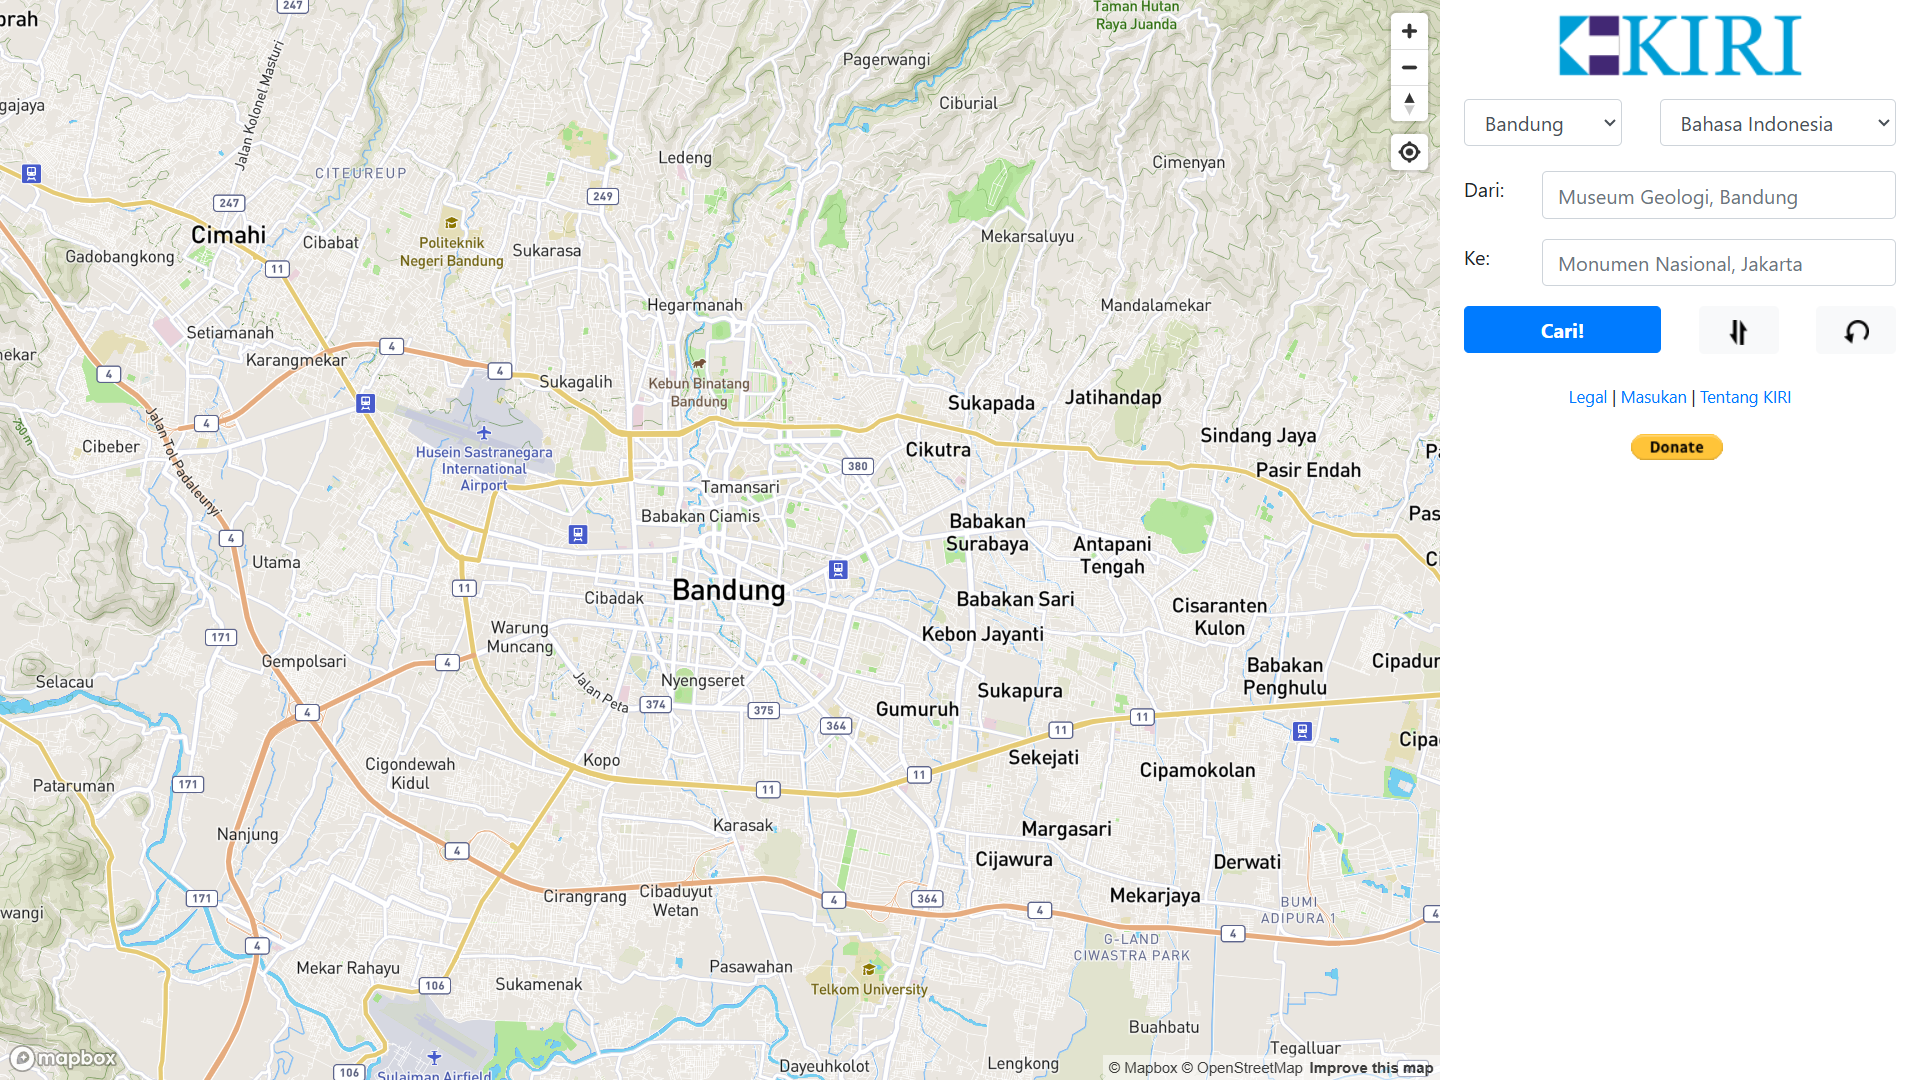
\includegraphics[width=1\textwidth]{Gambar/KIRI.png}  
	\caption{Tampilan halaman perangkat lunak KIRI}
	\label{fig:kiri} 
\end{figure}
\newpage
\noindent
KIRI akan memberikan informasi mengenai langkah-langkah yang harus ditempuh oleh pengguna yang akan bepergian dari suatu tempat ke tempat tujuannya, mulai dari seberapa jauh pengguna harus berjalan untuk menaiki angkot yang bersangkutan, di mana pengguna harus naik atau turun angkot tersebut, seberapa jauh lagi pengguna harus berjalan sampai ke lokasi tujuan, dan seberapa lama estimasi waktu perjalanan yang akan ditempuh (lihat Gambar \ref{fig:kiri2}).
\begin{figure}[H] 
	\centering  
	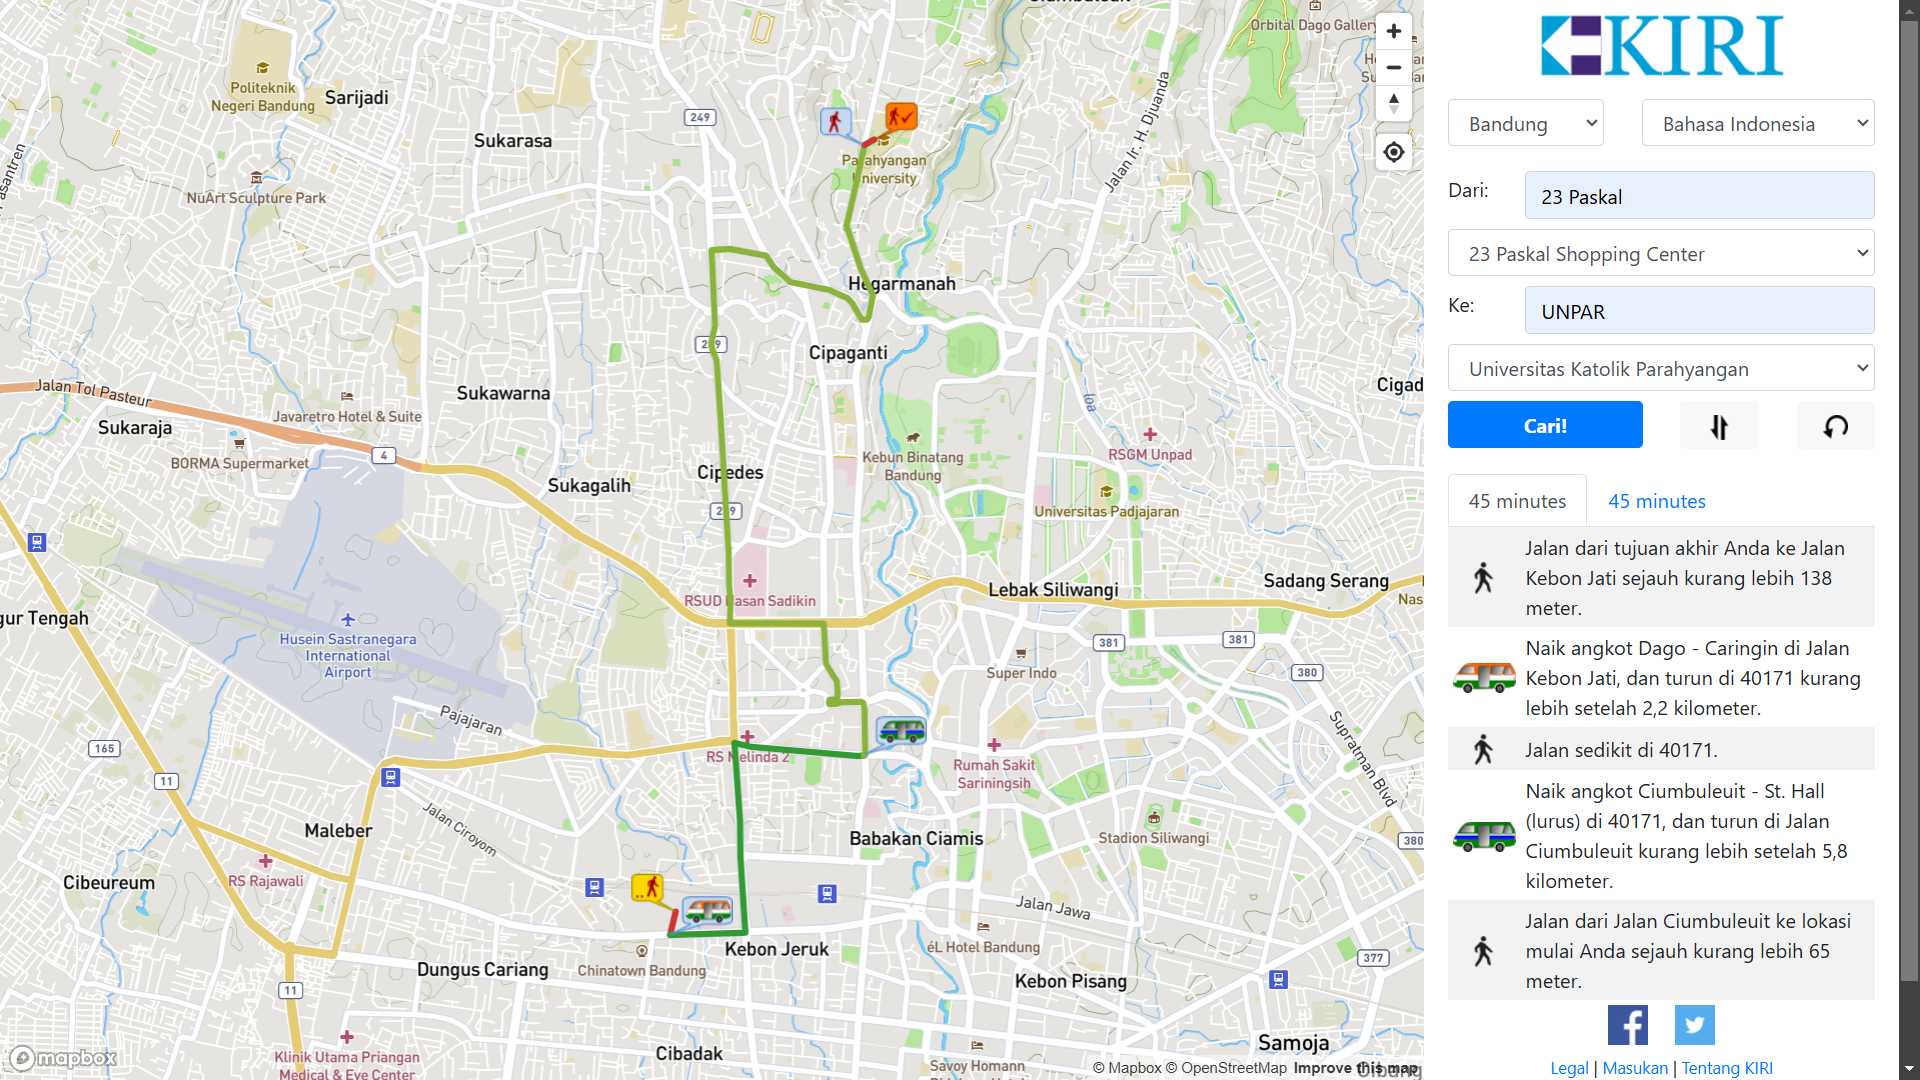
\includegraphics[width=1\textwidth]{Gambar/KIRI-2.png}  
	\caption{Tampilan perangkat lunak KIRI, setelah menerima masukan}
	\label{fig:kiri2} 
\end{figure}
\noindent
Arsitektur aplikasi KIRI terbagi menjadi dua bagian utama. Bagian \textit{frontend}, yang dinamakan Tirtayasa dan dibangun menggunakan bahasa pemrograman PHP serta mengandalkan basis data MySQL untuk menyimpan serta mengelola data. Selain itu, Tirtayasa juga menggunakan framework CodeIgniter 3. Saat menerima permintaan pencarian, Tirtayasa meneruskannya ke bagian \textit{backend}, yaitu NewMenjangan. Hasil dari NewMenjangan kemudian diformat agar dapat dibaca dengan baik oleh pengguna. Bagian ini diimplementasikan dalam bahasa pemrograman Java dan berperan penting dalam perhitungan rute optimal.\footnote{\url{https://ejournals.umn.ac.id/index.php/IJNMT/article/view/784}}
\\
NewMenjangan merupakan program \textit{daemon} yang berjalan secara otomatis saat server dinyalakan dan terus beroperasi hingga server dimatikan. \textit{Daemon} sendiri adalah program komputer yang berjalan dilatar belakang dan tidak berinteraksi langsung dengan pengguna\footnote{\url{https://www.ibm.com/docs/en/aix/7.1?topic=processes-}}. Pada saat eksekusi, NewMenjangan terhubung ke basis data MySQL untuk mengambil data rute angkot yang tersimpan dalam format LineString. LineString adalah salah satu tipe data geometris dalam MySQL yang mewakili satu atau lebih segmen garis yang terhubung. LineString terdiri dari urutan titik (\textit{point}) yang membentuk jalur atau lintasan\footnote{\url{https://dev.mysql.com/doc/refman/8.4/en/gis-linestring-property-functions.html}}. Setiap titik pada LineString merepresentasikan lokasi potensial untuk penumpang naik atau turun. Dari data tersebut, NewMenjangan membangun \textit{weighted graph} dalam memori (RAM) dalam bentuk \textit{adjacency list} dan melakukan prakomputasi. Setiap titik pada LineString menjadi akan \textit{node}, dan antara titik ke-i dan titik ke-(i+1) dihubungkan dengan \textit{edge}. Jika ada dua titik dari rute angkot berbeda yang berdekatan (jarak di bawah konstanta tertentu), maka dibuatkan juga \textit{edge}, yang menunjukkan kemungkinan seseorang dapat turun dari suatu angkot dan naik ke angkot lainnya untuk meneruskan perjalanan. 
\newpage
\noindent
Saat NewMenjangan menerima permintaan pencarian dari titik A ke titik B, kedua titik tersebut dijadikan \textit{node} sementara, dan dibuatkan \textit{edge} sementara ke \textit{node-node} yang sudah ada sebelumnya, jika jaraknya di bawah konstanta tertentu. Pencarian jarak terdekat pada graf tersebut dilakukan menggunakan algoritma Dijkstra versi teroptimasi (\textit{priority queue} dengan struktur data \textit{heap}). Proses ini dapat dilakukan secara paralel dengan aman (\textit{thread-safe}) tanpa mengubah graf utama.
\\
Pada saat ini algoritma yang digunakan KIRI masih terikat dengan algoritma Dijkstra. Oleh karena itu, pada tugas akhir ini akan diimplementasikan algoritma lainnya, yaitu algoritma A* dan Floyd-Warshall sebagai \textit{concrete strategy}. Selain itu, akan dilakukan juga penerapan arsitektur kelas \textit{strategy pattern} sehingga aplikasi KIRI akan menjadi lebih fleksibel dalam pemilihan algoritma \textit{shortest path} yang akan digunakan dan juga memudahkan apabila akan dilakukan perubahan atau perbaikan pada suatu algoritma yang digunakan.

\section{Rumusan Masalah}
\begin{enumerate}
    \item Bagaimana cara melakukan perubahan kode pada NewMenjangan untuk menerapkan \textit{strategy pattern}?
    \item Bagaimana mengimplementasikan algoritma A* dan Floyd-Warshall sebagai \textit{concrete strategy}?
\end{enumerate}

\section{Tujuan}
\begin{enumerate}
    \item Melakukan perubahan arsitektur kelas dengan menerapkan \textit{strategy pattern}.
    \item Melakukan implementasi algoritma A-star dan Floyd Warshall.
\end{enumerate}

\section{Detail Perkembangan Pengerjaan Tugas Akhir}
Detail bagian pekerjaan skripsi sesuai dengan rencana kerja/laporan perkembangan terkahir :
	\begin{enumerate}
		\item \textbf{Melakukan eksplorasi fungsi-fungsi dan cara kerja perangkat lunak KIRI.}\\
		{\bf Status :} Ada sejak rencana kerja skripsi.\\
		{\bf Hasil :} KIRI adalah sebuah aplikasi navigasi transportasi umum berbasis \textit{web} yang menyediakan rute antara dua lokasi geografis menggunakan transportasi publik. KIRI dirancang untuk melayani kebutuhan pengguna angkot di Bandung serta TransJakarta dan Commuterline di DKI Jakarta.
        \\ KIRI memberikan informasi detail mengenai rute perjalanan pengguna dari satu lokasi ke lokasi tujuan. Informasi yang disediakan meliputi seberapa jauh pengguna harus berjalan untuk mencapai titik naik angkot, lokasi tepat untuk naik atau turun angkot, jarak yang masih harus ditempuh dengan berjalan kaki hingga mencapai tujuan, serta estimasi waktu perjalanan yang akan dihabiskan.
        \\ Pada aplikasi kiri pengguna dapat memanfaatkan peta dunia yang tersedia untuk melihat lokasi secara keseluruhan, dengan opsi \textit{zoom in} dan \textit{zoom out} untuk memperbesar atau memperkecil tampilan peta, sehingga memudahkan navigasi. Dengan fitur lokasi atau GPS, KIRI juga dapat mendeteksi lokasi pengguna secara otomatis yang mempermudah penentuan titik awal perjalanan. Selain itu, pengguna dapat memilih kota tertentu seperti Jakarta atau Bandung untuk memfokuskan pencarian rute perjalanan di wilayah yang relevan.
        \\ KIRI juga menyediakan pilihan bahasa, yaitu bahasa Inggris atau bahasa Indonesia, sesuai dengan preferensi pengguna. Pengguna dapat memasukkan titik awal dan titik tujuan dengan dua cara, yaitu dengan mengetikkannya di kolom \textit{input} atau dengan mengeklik langsung lokasi yang diinginkan pada peta. Setelah itu, aplikasi memungkinkan pencarian rute perjalanan berdasarkan masukan tersebut, memberikan rekomendasi rute terbaik yang mencakup informasi jarak, waktu, dan petunjuk langkah demi langkah. Tampilan awal halaman KIRI dan juga tampilan setelah menerima masukan berupa lokasi awal dan lokasi tujuan dapat dilihat pada gambar \ref{fig:kiriawal} dan gambar \ref{fig:kiriinput}.
        \begin{figure}[h] 
    	\centering  
    	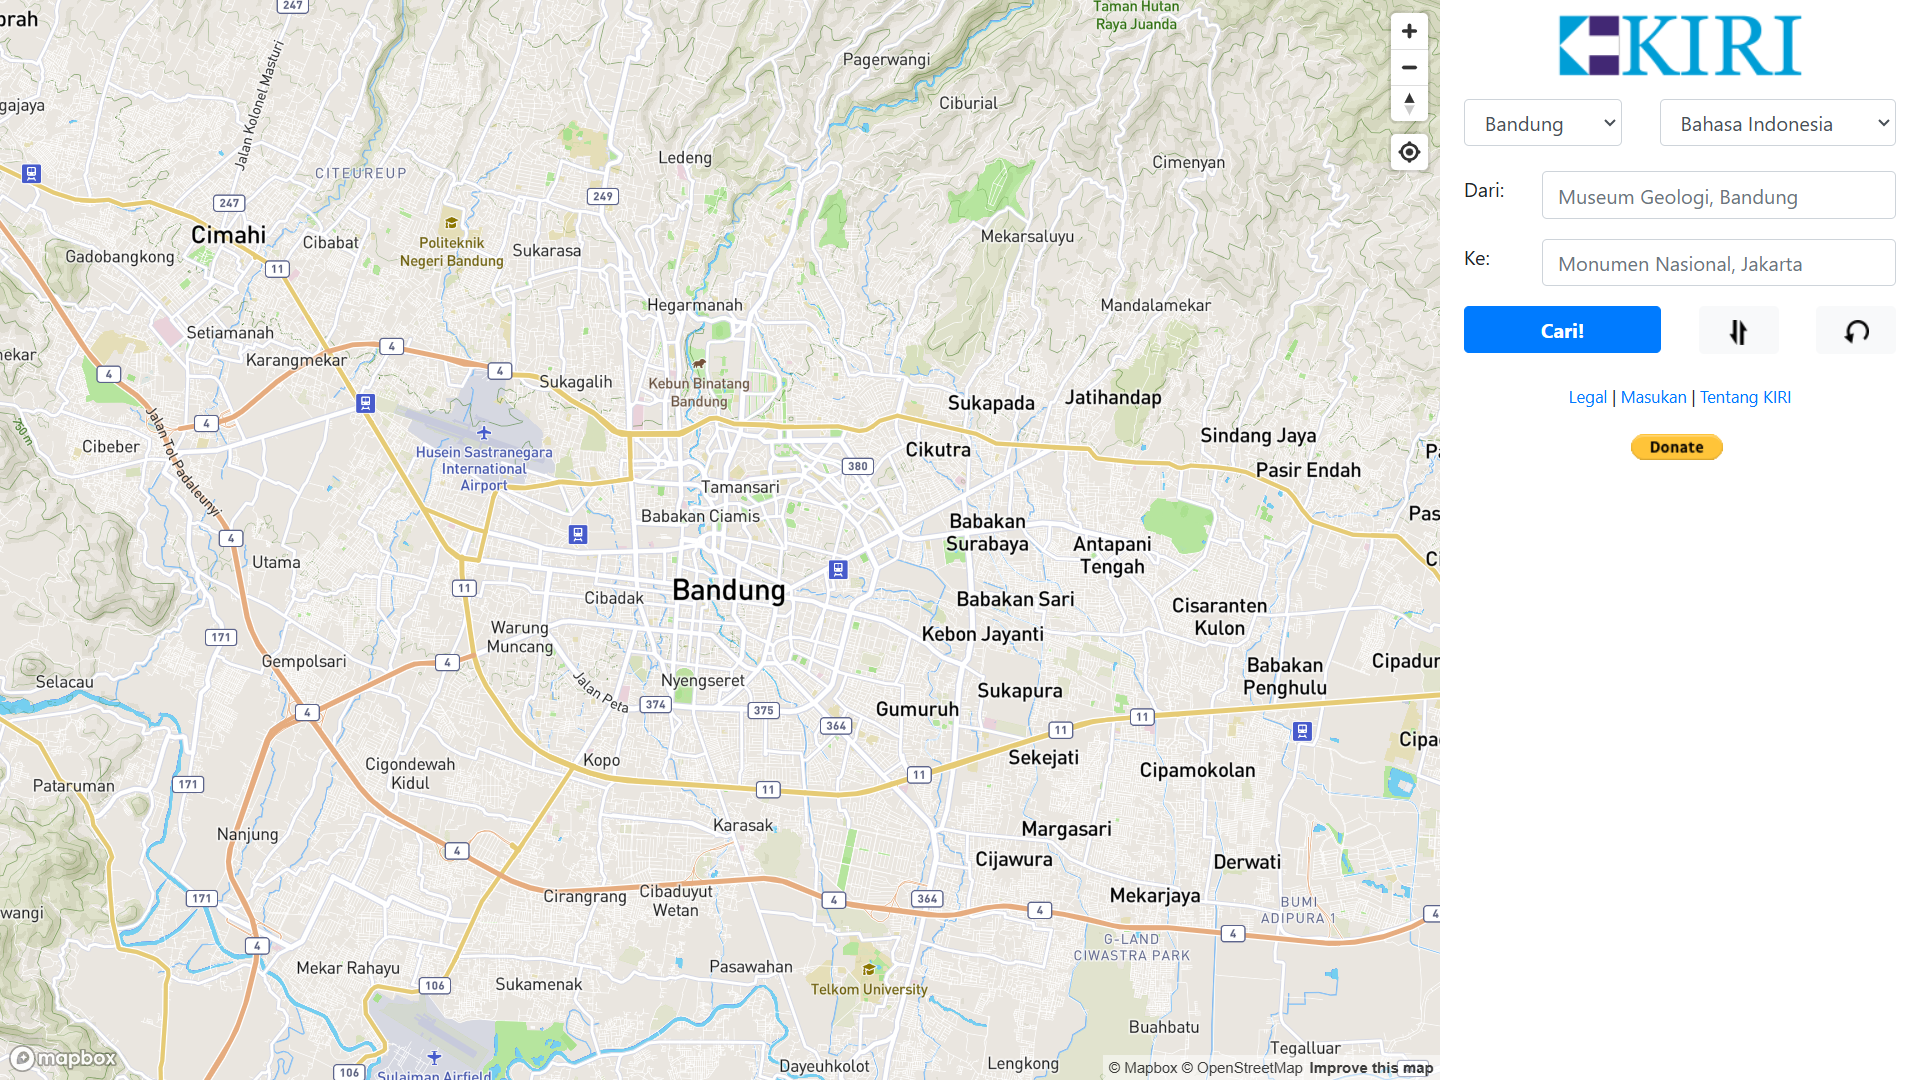
\includegraphics[width=1\textwidth]{Gambar/KIRI}  
    	\caption{Tampilan awal KIRI}
    	\label{fig:kiriawal} 
        \end{figure}

        \begin{figure}[H] 
    	\centering  
    	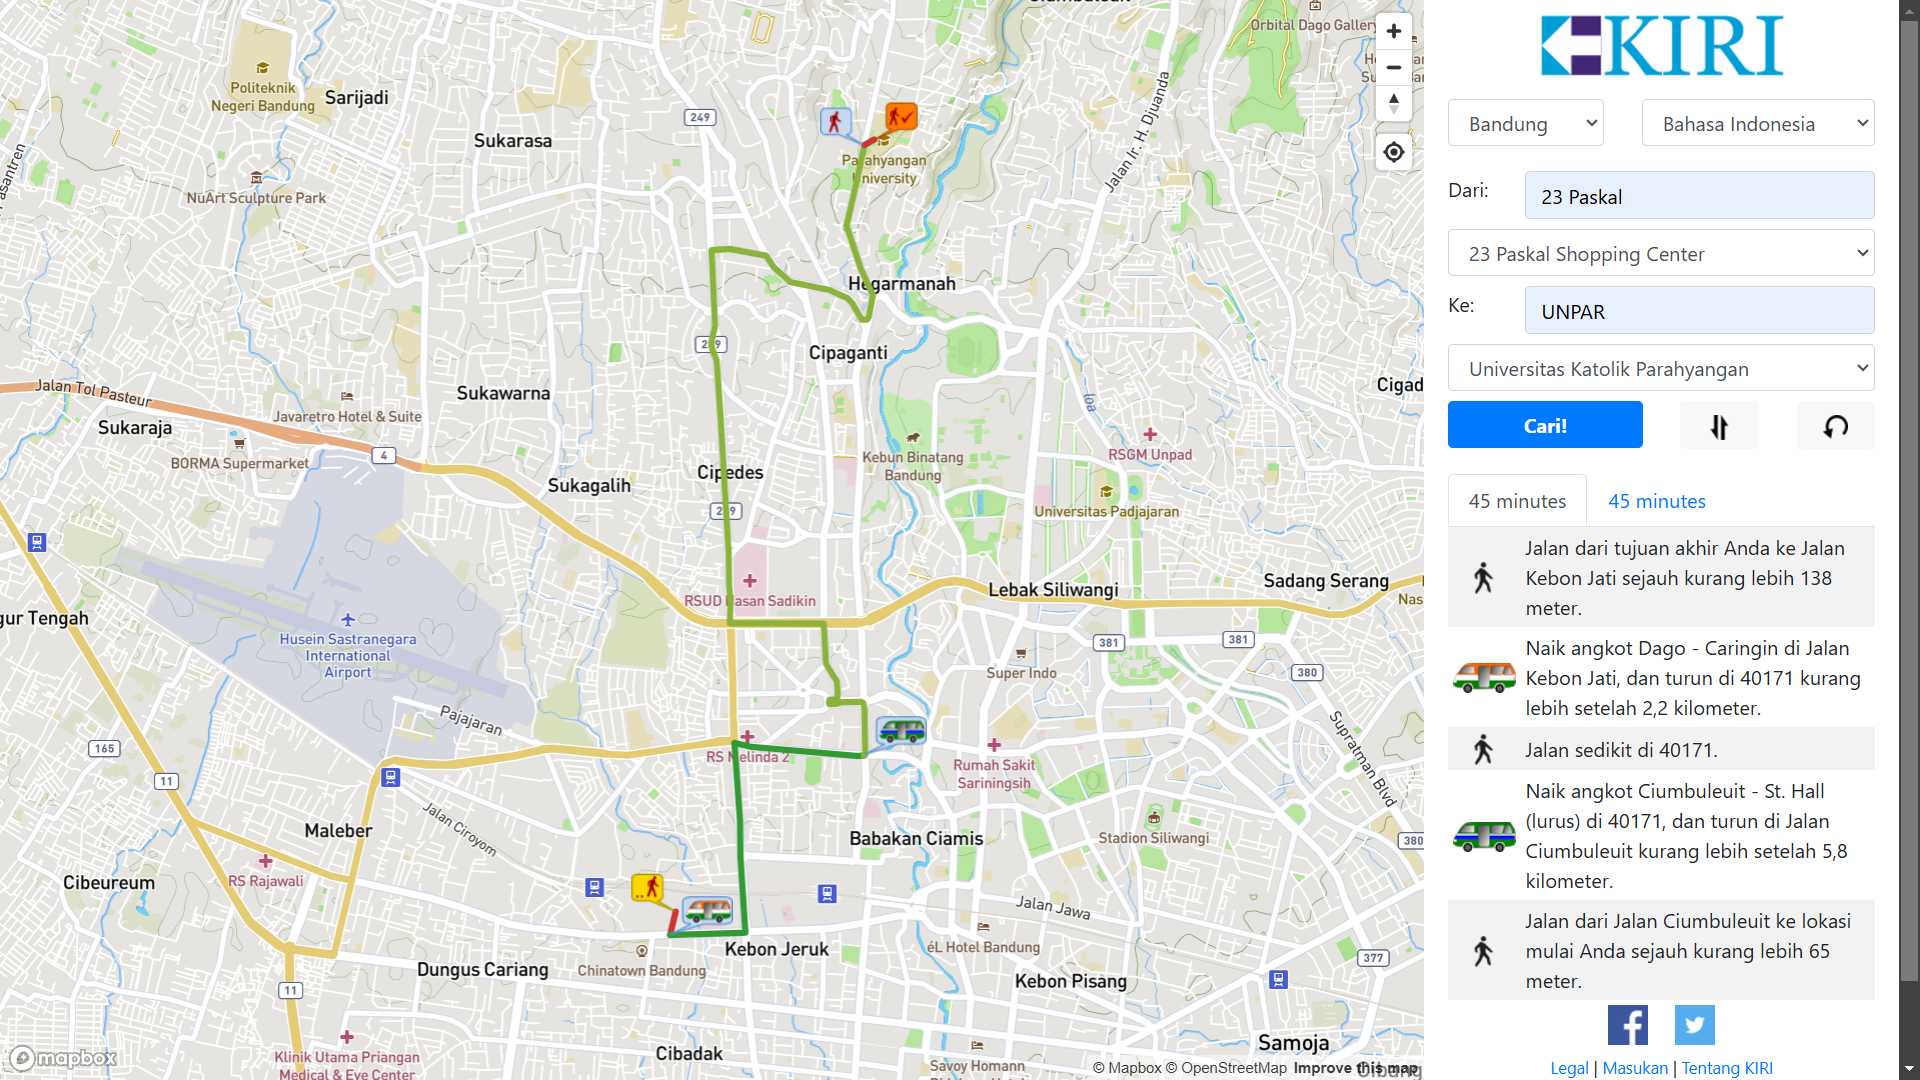
\includegraphics[width=1\textwidth]{Gambar/KIRI-2.png}  
    	\caption{Tampilan KIRI setelah menerima masukan}
    	\label{fig:kiriinput} 
        \end{figure}
\newpage
		\item \textbf{Mempelajari modul-modul yang terdapat pada Tirtayasa dan NewMenjangan.}\\
		{\bf Status :} Ada sejak rencana kerja skripsi.\\
		{\bf Hasil :} Tirtayasa dan NewMenjangan merupakan 2 bagian utama dari KIRI. Tirtayasa merupakan bagian \textit{frontend} yang dibangun menggunakan bahasa pemrograman PHP dan mengandalkan basis data MySQL untuk menyimpan serta mengelola data. Selain itu, Tirtayasa juga menggunakan framework CodeIgniter 3. Selanjutnya, yaitu NewMenjangan yang merupakan bagian \textit{backend} dari KIRI dan dibangun dengan bahasa pemrogrman Java serta digunakan untuk memproses permintaan navigasi. Komponen ini memuat semua jalur transportasi umum dalam bentuk graf dan menggunakan algoritma Dijkstra untuk menghitung rute optimal. Berikut struktur kelas dari NewMenjangan (Gambar \ref{fig:cd}).
        \begin{figure}[h] 
    	\centering  
    	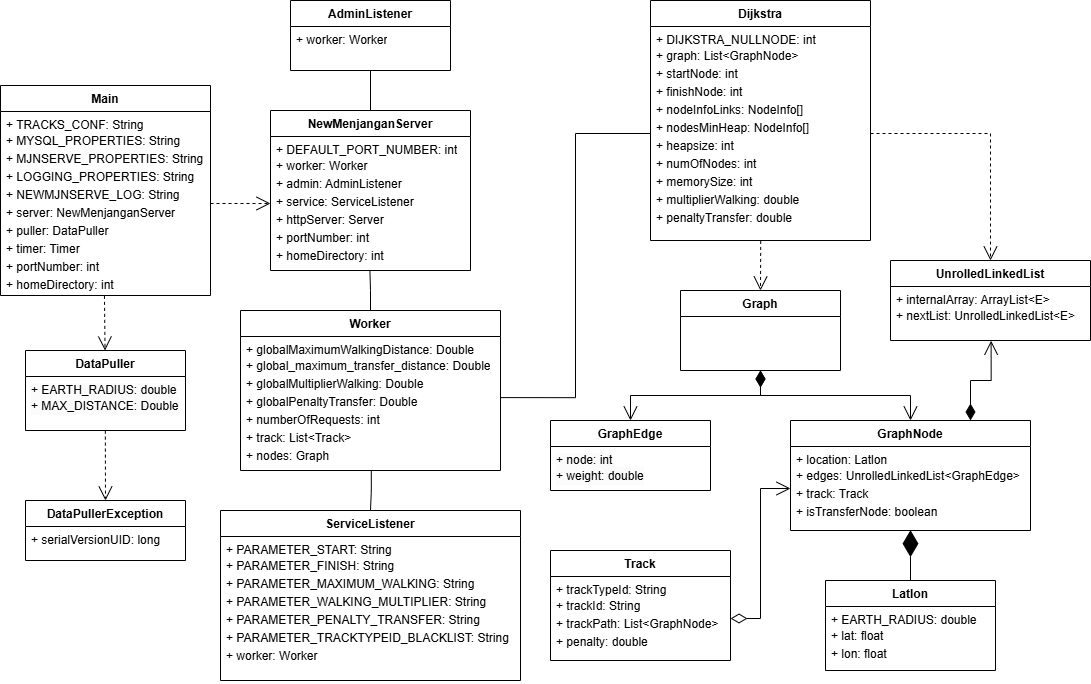
\includegraphics[width=0.8\textwidth]{Gambar/ClassDiagram.png}  
    	\caption{Struktur Kelas NewMenjangan}
    	\label{fig:cd} 
        \end{figure}

		\item \textbf{Mempelajari bahasa pemrograman PHP dan framework CodeIgniter 3.}\\
		{\bf Status :} Dihapuskan/tidak dikerjakan.\\
		{\bf Hasil :} Berdasarkan analisis singkat, bahasa pemrograman PHP dan framework CodeIgniter 3 merupakan bagian dari \textit{frontend} KIRI, yaitu Tirtayasa. Pada tugas akhir ini, penelitian lebih difokuskan ke bagian \textit{backend} KIRI (NewMenjangan) sehingga bahasa pemrograman PHP dan framework CodeIgniter 3 tidak didalami lebih jauh lagi.

		\item \textbf {Melakukan studi literatur mengenai penerapan arsitektur kelas \textit{straregy pattern}.}\\
		{\bf Status :} Ada sejak rencana kerja skripsi.\\
		{\bf Hasil :} Strategy Pattern merupakan salah satu pola desain perilaku yang dirancang untuk mendefinisikan serangkaian algoritma, mengenkapsulasi setiap algoritma, dan memungkinkan algoritma-algoritma tersebut untuk saling dipertukarkan. Pola ini memungkinkan algoritma untuk bervariasi. Dengan demikian, klien tidak perlu mengetahui detail implementasi dari algoritma yang digunakan, melainkan cukup berinteraksi melalui antarmuka umum yang disediakan oleh objek strategi.
        \\
        Pola ini sangat berguna ketika terdapat kebutuhan untuk mendukung berbagai varian algoritma dalam menyelesaikan tugas yang sama. Strategy Pattern memindahkan setiap algoritma ke dalam kelas terpisah, yang disebut sebagai \textit{concrete strategy}. Klien dapat memilih dan menentukan strategi yang sesuai ke dalam konteks pada waktu eksekusi, sehingga memberikan fleksibilitas yang tinggi dalam proses pengembangan perangkat lunak.
        \newpage
        Manfaat utama dari strategy pattern adalah kemampuannya untuk menghilangkan kompleksitas yang diakibatkan oleh penggunaan pernyataan kondisional yang rumit dalam kode, serta kemudahan dalam menambahkan atau mengganti algoritma tanpa perlu memodifikasi kode klien atau konteks. Namun, penerapan pola ini juga memiliki kelemahan, seperti meningkatnya jumlah kelas dalam sistem dan potensi timbulnya \textit{overhead} komunikasi antara konteks dan strategi. Oleh karena itu, penerapan strategy pattern sebaiknya dipertimbangkan dengan cermat, terutama dalam situasi di mana variasi algoritma memang diperlukan untuk memenuhi kebutuhan sistem.
        \\
        Berikut merupakan struktur dari strategy pattern (Gambar \ref{fig:struktursp}).
        \begin{figure}[h] 
    	\centering  
    	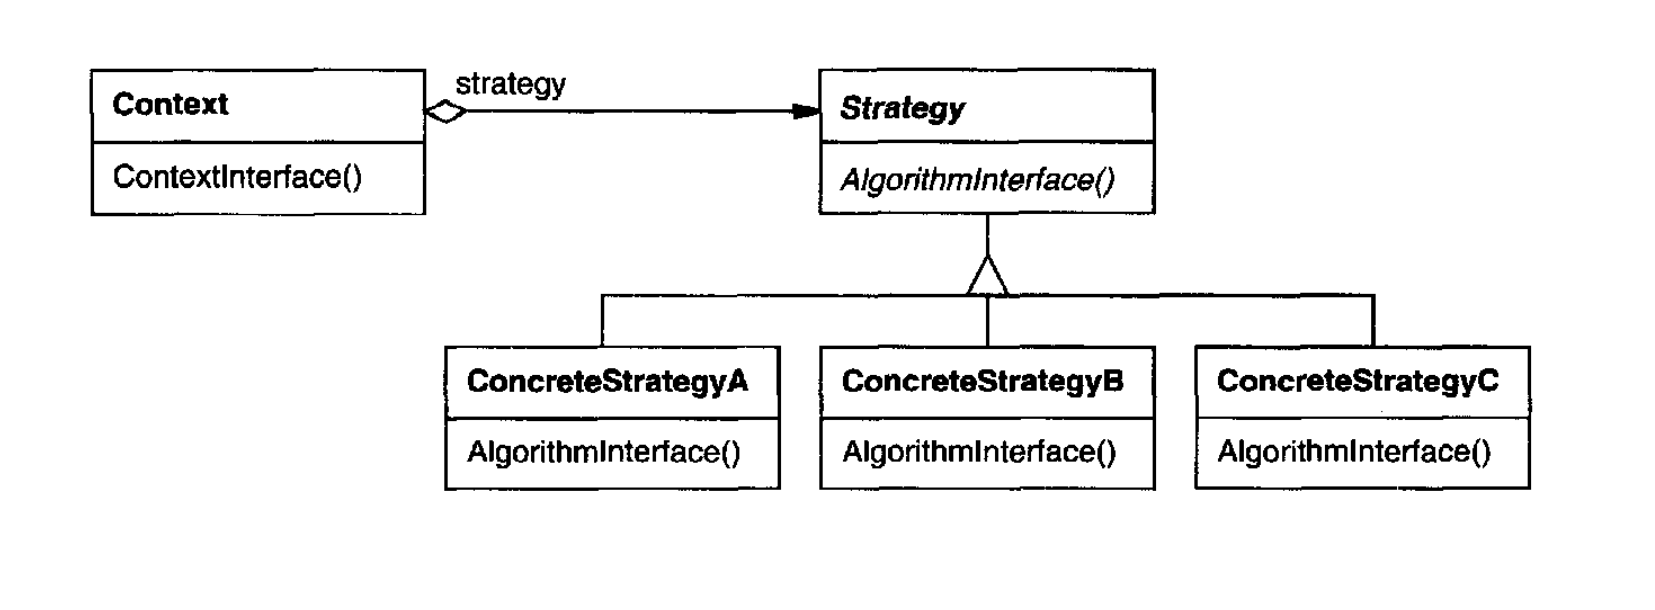
\includegraphics[width=1\textwidth]{Gambar/struktur-sp.png}  
    	\caption{Struktur Strategy Pattern}
    	\label{fig:struktursp} 
        \end{figure}

		\item \textbf{Melakukan studi literatur mengenai Graf.}\\
		{\bf Status :} Baru ditambahkan ketika pengerjaan TA 1.\\
		{\bf Hasil :} Graf ($G$) adalah struktur yang terdiri dari simpul (\textit{vertex}) dan sisi (\textit{edge}), dimana sisi menghubungkan pasangan simpul. Sebuah graf direpresentasikan sebagai pasangan $G=(V,E)$, dengan $V$ sebagai himpunan simpul dan $E$ sebagai himpunan sisi. Sisi diwakili oleh pasangan simpul yang terhubung. Graf dapat bersifat terarah atau tidak terarah.
        \\
        Simpul-simpul dalam graf dapat memiliki derajat tertentu, yaitu jumlah sisi yang menghubunginya. Sebuah graf disebut terhubung jika terdapat jalur antara setiap pasangan simpul. Jalur ini adalah urutan simpul yang dihubungkan oleh sisi. Selain itu, siklus adalah jalur tertutup di mana simpul awal dan akhir adalah sama. Teori graf juga mencakup konsep seperti pohon (graf terhubung tanpa siklus), graf bipartit (simpul dibagi menjadi dua himpunan yang saling bebas sisi), dan subgraf (bagian dari graf yang tetap mempertahankan struktur graf).
        \\
        Graf digunakan dalam berbagai hal, seperti jaringan komputer, rute transportasi, dan analisis hubungan sosial. Teori graf menyediakan dasar matematis untuk mempelajari struktur ini dan memberikan cara untuk memodelkan dan menyelesaikan masalah kompleks di berbagai bidang. 
        
		\item \textbf{Mempelajari cara kerja algoritma Dijkstra, A-star, dan Floyd Warshall.}\\
		{\bf Status :} Ada sejak rencana kerja skripsi.\\
		{\bf Hasil :} Algoritma Dijkstra, Floyd-Warshall, dan A* merupakan sebuah algoritma \textit{shortest path} yang dirancang untuk menemukan lintasan terpendek antara dua titik dalam sebuah graf. Ketiga algoritma tersebut merupakan algoritma yang akan diimplementasikan pada perangkat lunak KIRI sebagai \textit{concrete strategy}. Berikut pembahasan cara kerja algoritma yaitu Dijkstra, Floyd-Warshall, dan A*.
        \newpage
        \begin{itemize}
            \item \textbf{Algoritma Dijkstra}
            \\ Algoritma Dijkstra merupakan sebuah algoritma untuk menyelesaikan masalah \textit{single-source shortest path}, yaitu menemukan jalur terpendek dari satu titik asal ke semua titik lainnya dalam sebuah graf berarah dengan bobot tepi non-negatif. Algoritma ini menggunakan sebuah struktur \textit{min-priority queue} (antrean prioritas minimum) yang menyimpan titik-titik dengan prioritas sesuai dengan perkiraan jarak terpendek dari titik asal.
            \begin{figure}[H] 
            	\centering  
            	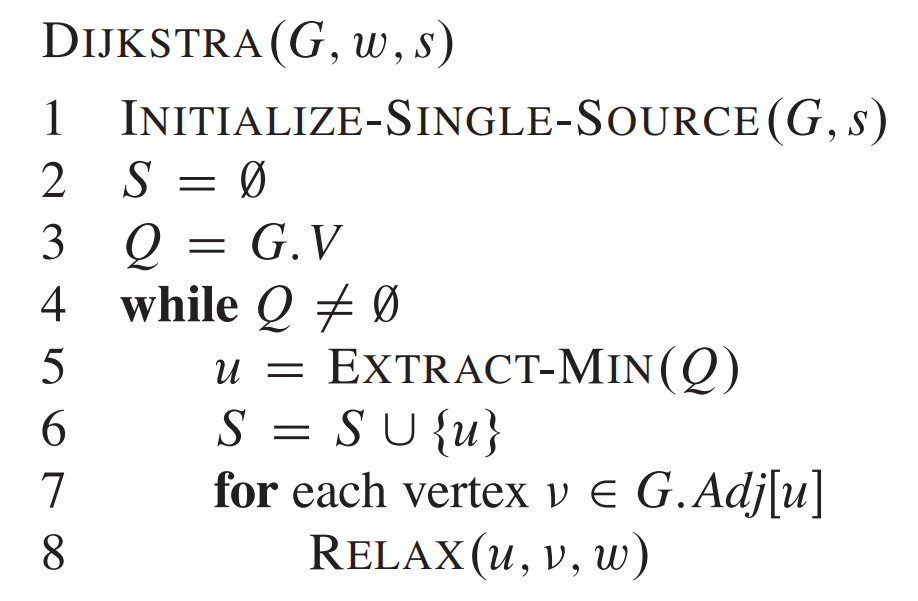
\includegraphics[width=0.5\textwidth]{Gambar/dijkstra.png}  
            	\caption{Pseudocode Algoritma Dijkstra}
            	\label{fig:pseudocodedijkstra} 
            \end{figure}
            \noindent
            \\
            Gambar \ref{fig:pseudocodedijkstra} merupakan pseudocode dari algoritma Dijkstra. Pada pseudocode terdapat beberapa atribut diantarnya, yaitu $G$ yang merepresentasikan graf, $w$ merupakan bobot yang menyatakan jarak atau biaya antar dan $s$ merepresentasikan simpul sumber yang merupakan titik awal pencarian. Selain itu, $S$ merepresentasikan kumpulan simpul yang sudah diproses yang diawal diinisialisasikan kosong, sedangkan $Q$ merepresentasikan kumpulan simpul yang belum diproses, kemudian $u$ merepresentasikan simpul yang sedang diproses dan $v$ merepresentasikan simpul tetangga dari $u$. Algoritma Dijkstra dimulai dengan menginisialisasi perkiraan jarak terpendek dari titik asal $s$ ke semua titik lain, kecuali $s$ itu sendiri yang diinisialisasi dengan jarak 0 dan juga semua simpul dimasukkan ke dalam \textit{min-priority queue} ($Q$), di mana prioritas ditentukan berdasarkan jarak terpendek yang diketahui. Selanjutnya, algoritma memproses simpul-simpul satu per satu dengan memilih simpul $u$ dari $Q$ yang memiliki jarak terpendek. Simpul tersebut kemudian ditambahkan ke dalam himpunan $S$.
            \\
            Setelah simpul $u$ diproses, algoritma akan memeriksa semua tetangga $v$ dari $u$. Untuk setiap tetangga, algoritma melakukan proses \textit{relaksasi}, yaitu membandingkan jarak saat ini ke $v$ dengan jarak yang melewati $u$. Jika jalur melalui $u$ memberikan jarak yang lebih pendek, jarak ke $v$ diperbarui dengan jarak baru tersebut, dan simpul pendahulu $v$ diatur menjadi $u$. Proses ini memastikan bahwa jalur terpendek ditemukan secara bertahap melalui iterasi. Algoritma akan terus berjalan hingga semua simpul telah diproses atau antrean $Q$ kosong. Hasil akhir berupa jarak terpendek dari simpul sumber $s$ ke setiap simpul lain dalam graf.

            \item \textbf{Algoritma Floyd-Warshall}
            \\ Algoritma Floyd-Warshall merupakan sebuah algoritma untuk menyelesaikan masalah jalur terpendek untuk semua pasangan titik dalam graf berarah dengan menggunakan pendekatan pemrograman dinamis. Algoritma ini sangat berguna untuk graf yang memiliki bobot sisi negatif, selama tidak terdapat siklus dengan bobot negatif dalam graf tersebut. Pendekatan ini menghitung jalur terpendek antara semua pasangan titik dengan menggunakan tabel bobot antar titik dan mengulanginya secara bertahap untuk mencapai solusi optimal.
            \begin{figure}[H] 
            	\centering  
            	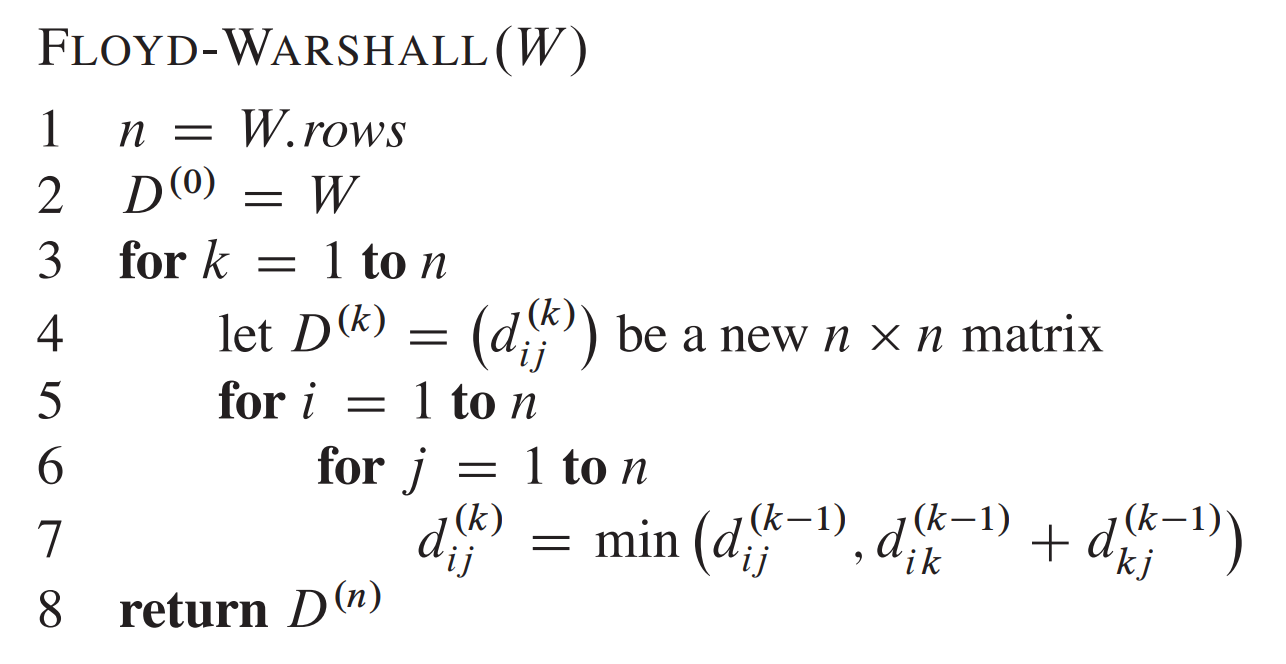
\includegraphics[width=0.7\textwidth]{Gambar/fw.png}  
            	\caption{Pseudocode Algoritma Floyd-Warshall}
            	\label{fig:pseudocodefw} 
            \end{figure}
            \noindent
            Gambar \ref{fig:pseudocodefw} merupakan pseudocode dari algoritma Floyd-Warshall. Pada pseudocode terdapat beberapa atribut diantarnya, yaitu $W$ yang merupakan sebuah matriks berbobot berukuran $n*n$ dan mewakili bobot dari setiap sisi pada graf, $D^{(0)}$ atau $D^{(k)}$ merupakan Matriks berukuran $n*n$ pada iterasi ke-$k$, $n$ merepresentasikan banyaknya simpul dalam graf, diperoleh dari jumlah baris dari matriks $W$. Selain itu, terdapat $d_{ij}^{(k)}$ yang merupakan elemen dari matriks $D^{(k)}$ yang menunjukkan jarak terpendek antara simpul $i$ dan $j$ pada iterasi ke-$k$. Algoritma Floyd-Warshall dimulai dengan menginisialisasi $n$ yang diinisialisasi dengan nilai baris pada matriks $W$ dan juga $D^{(0)}$ yang diinisialisasi dengan matriks $W$. 
            \\
            Selama $n$ iterasi, algoritma memperbarui matriks jarak terpendek dengan mempertimbangkan kemungkinan jalan melalui simpul antara $\{1,2,...,k\}$. Pada setiap langkah, algoritma memeriksa apakah jarak dari $i$ ke $j$ dapat diperpendek dengan melalui simpul $k$, dibandingkan dengan jarak langsung antara $i$ dan $j$. Proses ini menghasilkan solusi optimal, di mana 
            $D^{(n)}$ mencakup semua jarak terpendek yang memungkinkan.Algoritma Floyd-Warshall memiliki kompleksitas waktu $O(n^3)$ karena terdiri dari tiga \textit{looping} untuk semua titik dalam graf.

            \item \textbf{Algoritma A*}
            \\ Algoritma A* adalah metode pencarian yang meminimalkan estimasi total biaya solusi dengan menggabungkan dua fungsi, yaitu $g(n)$ dan $h(n)$ Fungsi $g(n)$ menghitung biaya aktual dari titik awal hingga simpul $n$, sedangkan $h(n)$ memperkirakan biaya tersisa dari $n$ ke tujuan. Kombinasi ini menghasilkan $f(n) = g(n) + h(n)$, yang memberikan perkiraan total biaya solusi jika rute melalui simpul $n$. Algoritma ini biasanya dipilih karena dapat mencapai solusi yang optimal dan lengkap, terutama jika fungsi heuristik $h(n)$ memenuhi kriteria tertentu.
            \\
            Kondisi utama yang diperlukan agar algortima A* memberikan solusi optimal adalah heuristik $h(n)$ yang bersifat \textit{admissible}, yaitu tidak pernah melebih-lebihkan biaya ke tujuan, dan \textit{consistent} atau \textit{monotonic}, di mana nilai $h$ tidak menurun di sepanjang jalur. Dengan adanya heuristik yang memenuhi syarat ini, algoritma A* dapat menghindari eksplorasi simpul-simpul yang tidak relevan, mengurangi waktu dan memori yang dibutuhkan.
            \\
            Terdapat kendala utama dari algoritma A*, yaitu penggunaan memori yang besar karena algoritma ini perlu menyimpan semua simpul yang telah dihasilkan. Untuk mengatasi hal ini, terdapat varian A* seperti \textit{Iterative-Deepening A*} (IDA*) yang mengurangi kebutuhan memori tanpa mengorbankan optimalitas solusi, dengan biaya eksekusi yang sedikit lebih tinggi.
        \end{itemize}
\newpage
		\item \textbf{Mengubah implementasi algoritma Dijkstra yang sudah ada ke dalam \textit{strategy pattern}.}\\
		{\bf Status :} Ada sejak rencana kerja skripsi. \\
		{\bf Hasil :} Implementasi belum terselesaikan karena pengerjaan difokuskan terlebih dahulu ke dokumen tugas akhir.

		\item \textbf{Menulis sebagian dokumen skripsi, yaitu Bab 1, 2, dan 3.} \\
		{\bf Status :} Ada sejak rencana kerja skripsi.\\
		{\bf Hasil :} Dokumen skripsi bab 1 berisikan latar belakang, rumusan masalah, tujuan, batasan masalah, metodologi, dan sistematika pembahasan. Untuk saat ini batasan masalah masih belum diisi dan akan dilakukan ketika TA 2. Bab 2 berisikan penjelasan teori-teori yang diperlukan untuk penelitian, diantranya, yaitu KIRI, Design Pattern dan Strategy Pattern, MySQL dan \textit{LineString}, dan Algoritma \textit{Shortest Path} yang terdiri dari algoritma Dijkstra, algoritma Floyd-Warshall, dan algoritma A*. Kemudian, Bab 3 berisikan analisis sistem kini yang menjelaskan mengenai struktur kelas pada NewMenjangan dan juga analisis untuk sistem usulan, yang dimana akan diimplementasikan strategy pattern dengan algoritma Dijkstra, algoritma Floyd-Warshall, dan algoritma A* akan menjadi \textit{concrete strategy}. Selain itu, akan diimplementasikan juga algoritma Floyd-Warshall, dan algoritma A* karena untuk saat ini hanya algoritma Dijkstra saja yang baru diimplementasikan.
	\end{enumerate}

\section{Pencapaian Rencana Kerja}
Langkah-langkah kerja yang berhasil diselesaikan dalam Tugas Akhir 1 ini adalah sebagai berikut:
\begin{enumerate}
\item Melakukan eksplorasi fungsi-fungsi dan cara kerja perangkat lunak KIRI.
\item Mempelajari modul-modul yang terdapat pada Tirtayasa dan NewMenjangan.
\item Melakukan studi literatur mengenai penerapan arsitektur kelas straregy pattern.
\item Melakukan studi literatur mengenai graf.
\item Mempelajari cara kerja algoritma Dijkstra, A*, dan Floyd Warshall.
\item Menulis sebagian dokumen skripsi, yaitu Bab 1, 2, dan 3.
\end{enumerate}

\vspace{1cm}
\centering Bandung, \tanggal\\
\vspace{2cm} \nama \\ 
\vspace{1cm}

Menyetujui, \\
\ifdefstring{\jumpemb}{2}{
\vspace{1.5cm}
\begin{centering} Menyetujui,\\ \end{centering} \vspace{0.75cm}
\begin{minipage}[b]{0.45\linewidth}
% \centering Bandung, \makebox[0.5cm]{\hrulefill}/\makebox[0.5cm]{\hrulefill}/2013 \\
\vspace{2cm} Nama: \pembA \\ Pembimbing Utama
\end{minipage} \hspace{0.5cm}
\begin{minipage}[b]{0.45\linewidth}
% \centering Bandung, \makebox[0.5cm]{\hrulefill}/\makebox[0.5cm]{\hrulefill}/2013\\
\vspace{2cm} Nama: \pembB \\ Pembimbing Pendamping
\end{minipage}
\vspace{0.5cm}
}{
% \centering Bandung, \makebox[0.5cm]{\hrulefill}/\makebox[0.5cm]{\hrulefill}/2013\\
\vspace{2cm} Nama: \pembA \\ Pembimbing Tunggal
}
\end{document}
